\documentclass[11pt, a4paper, twoside, titlepage]{article}
\usepackage[a4paper]{geometry}
\usepackage[T1]{fontenc}
\usepackage[utf8]{inputenc}
\usepackage[french]{babel}
\usepackage{graphicx}
\usepackage{caption}
\usepackage{listings}
\usepackage{color}

\geometry{hscale=0.75, vscale=0.85, centering}
\font\titlefont=cmr12 at 24pt
\graphicspath{ {images/} }

\definecolor{mygreen}{rgb}{0,0.6,0}
\definecolor{mygray}{rgb}{0.5,0.5,0.5}
\definecolor{mymauve}{rgb}{0.58,0,0.82}
\definecolor{mycontrol}{rgb}{0.98,0.98,0.98}

\lstset{ 
  backgroundcolor=\color{mycontrol}, % choose the background color; you must add \usepackage{color} or \usepackage{xcolor}; should come as last argument
  basicstyle=\footnotesize,          % the size of the fonts that are used for the code
  breakatwhitespace=false,           % sets if automatic breaks should only happen at whitespace
  breaklines=true,                   % sets automatic line breaking
  captionpos=b,                      % sets the caption-position to bottom
  commentstyle=\color{mygreen},      % comment style
  deletekeywords={...},              % if you want to delete keywords from the given language
  escapeinside={\%*}{*)},            % if you want to add LaTeX within your code
  extendedchars=true,                % lets you use non-ASCII characters; for 8-bits encodings only, does not work with UTF-8
  frame=single,	                     % adds a frame around the code
  keepspaces=true,                   % keeps spaces in text, useful for keeping indentation of code (possibly needs columns=flexible)
  keywordstyle=\color{blue},         % keyword style
  language=caml,                     % the language of the code
  morekeywords={*,...},              % if you want to add more keywords to the set
  numbers=none,                      % where to put the line-numbers; possible values are (none, left, right)
  numbersep=5pt,                     % how far the line-numbers are from the code
  numberstyle=\tiny\color{mygray},   % the style that is used for the line-numbers
  rulecolor=\color{black},           % if not set, the frame-color may be changed on line-breaks within not-black text (e.g. comments (green here))
  showspaces=false,                  % show spaces everywhere adding particular underscores; it overrides 'showstringspaces'
  showstringspaces=false,            % underline spaces within strings only
  showtabs=false,                    % show tabs within strings adding particular underscores
  stepnumber=2,                      % the step between two line-numbers. If it's 1, each line will be numbered
  stringstyle=\color{mymauve},       % string literal style
  tabsize=4,	                     % sets default tabsize to 2 spaces
  title=\lstname                     % show the filename of files included with \lstinputlisting; also try caption instead of title
}

\begin{document}

\title{{\titlefont Projet d'architecture matérielle}\\ARMAgeddon\thanks{J'aime les jeux de mots}}
\author{Pierre KOEBELIN}
\date{\today}
\maketitle

\begin{abstract}
L’objectif de ce projet était la réalisation d’un mini-processeur dans Diglog. Pour ce faire, nous devions nous appuyer sur le jeu d'instructions d'un processeur MIPS, que nous avons implémenté dans le logiciel Diglog\ldots\\
\\
Les instructions qui ont été implémentées sont:
\begin{itemize}
        \item{\texttt{nop}}
        \item{\texttt{ldi}}
        \item{\texttt{nop}}
        \item{\texttt{lsr}: une version simpléfiée qui ne décale que d'un bit}
        \item{\texttt{or} avec prédicat}
        \item{\texttt{and} avec prédicat}
        \item{\texttt{addi}}
        \item{\texttt{subi}}
        \item{\texttt{add} avec prédicat}
        \item{\texttt{sub} avec prédicat}
        \item{\texttt{cmpi}}
        \item{\texttt{cmp} avec prédicat}
        \item{\texttt{out}}
        \item{\texttt{in}}
        \item{\texttt{jeq}}
        \item{\texttt{jle}}
        \item{\texttt{jlt}}
        \item{\texttt{jne}}
        \item{\texttt{jmp}}
\end{itemize}
\end{abstract}

\tableofcontents

\newpage
\section{ALU}
\paragraph{}
Cet ALU permet de faire de nombreuses opérations sur des entiers sur 8 bits, comme l'addition et la soustraction en signée et non signée, ainsi que le complément à 1, l'incrémentation, l'opposé et les ET et OU binaires.\\
\\
\centerline{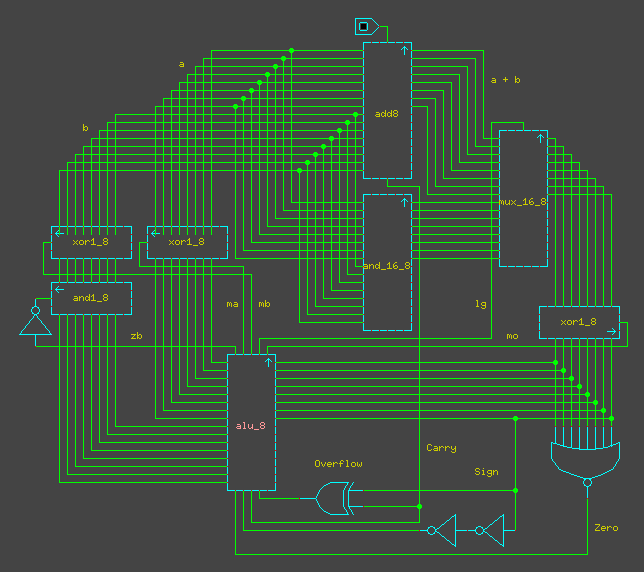
\includegraphics[width=.8\textwidth]{alu_8}}
\captionof{figure}{ALU à 5 bits de contrôle et 4 bits de sortie}

\paragraph{Bits de contrôle et de sortie}
Il prend en entrée deux entiers codés sur 8 bits et est géré par 5 bits de contrôle: \texttt{zb}, \texttt{ma}, \texttt{mb}, \texttt{lg} et \texttt{mo}. Il propose en sortie le résultat de l'opération sur 8 bits, ainsi que 4 bits de sortie: \texttt{Zero}, \texttt{Sign}, \texttt{Carry} et \texttt{Overflow}.

\subsection{Bits de contrôle}
\paragraph{}
Ces bits de contrôle sont au nombre de cinq et permettent de réaliser différentes opérations sur les entrées \texttt{a} et \texttt{b}.\\
\\
\centerline{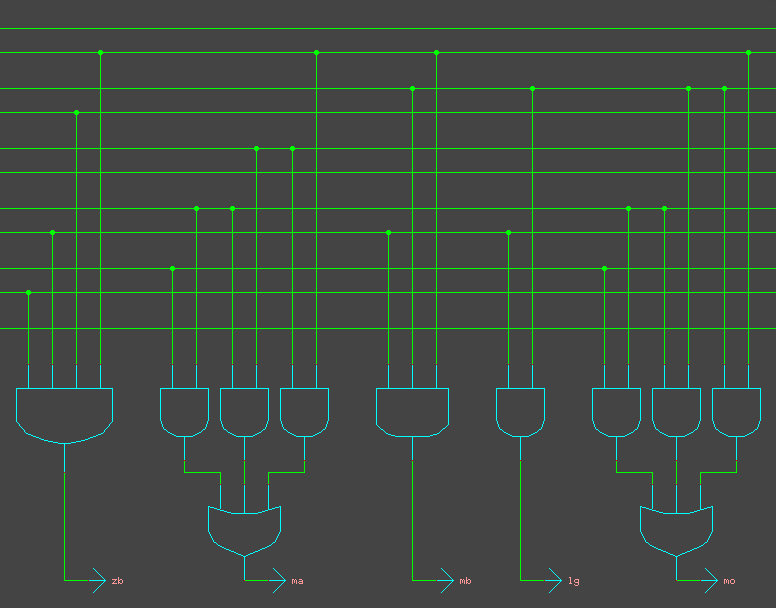
\includegraphics[width=.8 \textwidth]{log_alu}}
\captionof{figure}{Calcul des bits de contrôle de l'ALU}
\paragraph{}
\subsubsection{\texttt{zb}}
Ce bit de contrôle gère le bloc \texttt{and1\_8} situé sur les bits de \texttt{b}, et permet de mettre \texttt{b} à 0 ou non avant de passer par le bloc \texttt{xor1\_8}.

\subsubsection{\texttt{ma}}
Ce bit de contrôle gère le bloc \texttt{xor1\_8} situé sur les bits de \texttt{a}, et permet de donner son complément à 1 avant d'être utilisé par \texttt{add8} et \texttt{and\_16\_8}.

\subsubsection{\texttt{mb}}
Ce bit de contrôle gère le bloc \texttt{xor1\_8} situé sur les bits de \texttt{b}, et permet de donner son complément à 1 avant d'être utilisé par \texttt{add8} et \texttt{and\_16\_8}.

\subsubsection{\texttt{lg}}
Ce bit de contrôle gère le multiplexeur \texttt{mux\_16\_8} permettant de retourner le résultat de \texttt{add8} ou celui de \texttt{and\_16\_8}.

\subsubsection{\texttt{mo}}
Ce bit de contrôle gère le bloc \texttt{xor1\_8} situé après le multiplexeur \texttt{mux\_16\_8}, et permet retourner le résultat de \texttt{add8} et \texttt{and\_16\_8} ou son complément à 1.\\
\\
Voici le tableau répertoriant les valeurs des bits de contrôle pour chaque instruction:
\begin{center}
	\ttfamily
	\begin{tabular}{|c|c|c|c|c|c|c|c|}
		\hline
		instr	& op & flags & zb & ma & mb & lg & mo \\
		\hline
				& abc & de &&&&& \\
		\hline
		nop		& 000 & 00 & X & X & X & X & X \\
		ldi		& 000 & 01 & X & X & X & X & X \\
				& 000 & 10 & X & X & X & X & X \\
				& 000 & 11 & X & X & X & X & X \\
		\hline
		not		& 001 & 00 & 1 & 1 & X & X & 0 \\
		lsr		& 001 & 01 & 0 & 0 & 0 & 0 & 0 \\
		or		& 001 & 10 & 0 & 1 & 1 & 1 & 1 \\
		and		& 001 & 11 & 0 & 0 & 0 & 1 & 0 \\
		\hline
		addi	& 010 & 00 & 0 & 0 & 0 & 0 & 0 \\
		add		& 010 & 01 & 0 & 0 & 0 & 0 & 0 \\
		subi	& 010 & 10 & 0 & 1 & 0 & 0 & 1 \\
		sub		& 010 & 11 & 0 & 1 & 0 & 0 & 1 \\
		\hline
		muli	& 011 & 00 & X & X & X & X & X \\
		mul		& 011 & 01 & X & X & X & X & X \\
		compi	& 011 & 10 & 0 & 1 & 0 & 0 & 1 \\
		comp	& 011 & 11 & 0 & 1 & 0 & 0 & 1 \\
		\hline
		st		& 100 & 00 & 0 & 0 & 0 & 0 & 0 \\
		ld		& 100 & 01 & 0 & 0 & 0 & 0 & 0 \\
		out		& 100 & 10 & X & X & X & X & X \\
		in		& 100 & 11 & X & X & X & X & X \\
		\hline
		jr		& 101 & 00 & X & X & X & X & X \\
				& 101 & 01 & X & X & X & X & X \\
				& 101 & 10 & X & X & X & X & X \\
				& 101 & 11 & X & X & X & X & X \\
		\hline
		jeq		& 110 & 00 & 0 & 1 & 0 & 0 & 1 \\
		jle		& 110 & 01 & 0 & 1 & 0 & 0 & 1 \\
		jlt		& 110 & 10 & 0 & 1 & 0 & 0 & 1 \\
		jne		& 110 & 11 & 0 & 1 & 0 & 0 & 1 \\
		\hline
		jmp		& 111 & 00 & X & X & X & X & X \\
		jmp		& 111 & 01 & X & X & X & X & X \\
		jmp		& 111 & 10 & X & X & X & X & X \\
		jmp		& 111 & 11 & X & X & X & X & X \\
		\hline
	\end{tabular}
\end{center}
\paragraph{}
On peut ainsi obtenir le tableau de Carnot suivant:
\begin{center}
	\ttfamily
	\large
	\begin{tabular}{|c|c|c|c|c|c|}
		\hline
		& de & 00 & 01 & 11 & 10 \\
		\hline
		abc &&&&& \\
		\hline 
		000 && X X X X X & X X X X X & X X X X X & X X X X X \\
		\hline 
		001 && 1 1 X X 0 & 0 0 0 0 0 & 0 0 0 1 0 & 0 1 1 1 1 \\
		\hline 
		011 && X X X X X & X X X X X & 0 1 0 0 1 & 0 1 0 0 1 \\
		\hline 
		010 && 0 0 0 0 0 & 0 0 0 0 0 & 0 1 0 0 1 & 0 1 0 0 1\\
		\hline 
		110 && 0 1 0 0 1 & 0 1 0 0 1 & 0 1 0 0 1 & 0 1 0 0 1 \\
		\hline 
		111 && X X X X X & X X X X X & X X X X X & X X X X X \\
		\hline 
		101 && X X X X X & X X X X X & X X X X X & X X X X X \\
		\hline 
		100 && 0 0 0 0 0 & 0 0 0 0 0 & 0 0 0 0 0 & 0 0 0 0 0 \\
		\hline
	\end{tabular}
\end{center}

\subsection{Bits de sortie}
\paragraph{}
Cest bits de sortie donnent des informations supplémentaires sur le déroulement de l'opération entre les entrées \texttt{a} et \texttt{b}.
	
\subsubsection{\texttt{Zero}}
Ce bit de sortie est à 1 lorsque le résultat de l'opération est nul. Dans le cas d'une soustraction, il indique donc une égalité.

\subsubsection{\texttt{Sign}}
Ce bit de sortie est identique au bit de poids le plus fort dans le résultat de l'opération, et indique son signe dans le cas d'un entier signé.

\subsubsection{\texttt{Carry}}
Ce bit de sortie est la retenue en sortie du bloc \texttt{add\_8}.

\subsubsection{\texttt{Overflow}}
Ce bit indique qu'il y a eu un Overflow.

\section{Modifications apportées au processeur}

\subsection{Introduction du registre \texttt{flags}}
\paragraph{}
Pour enregistrer le résultat d'une comparaison (instructions \texttt{cmpi} et \texttt{cmp}), on utilise un registre trois bits, dans lequel on écrit uniquement lorsqu'une de ces instructions est utilisée. Au début, les trois bits sont à \texttt{0}.\\
\\
\centerline{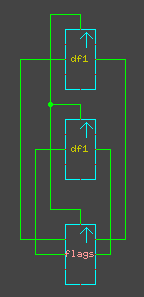
\includegraphics[scale=.8]{flags}}
\captionof{figure}{Registre \texttt{flags}}

\subsection{Gestion des prédicats}
\paragraph{}
Les instructions de type \texttt{1a} possèdent 2 bits actuellement inutilisés. Il est donc possible d'y attribuer des valeurs pour compléter ces instructions.\\
Le but ici est d'autoriser leur réalisation durant l'exécution selon le résultat de la dernière comparaison entre deux valeurs.\\
\\
\centerline{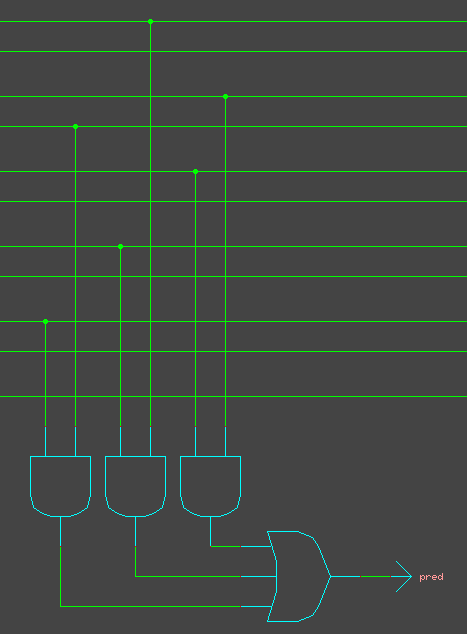
\includegraphics[width=.5 \textwidth]{log_pred}}
\captionof{figure}{Calcul du bit \texttt{pred}}
\paragraph{}
La sortie \texttt{pred} permet de savoir si on doit prendre en compte les deux bits de poids plus faibles afin de savoir si l'instruction doit être réalisée. Dans le cas contraire, il ne s'agit tout simplement pas du prédicat d'une instruction \texttt{1a}.

\subsection{Comparaison et calcul du bit \texttt{op}}
\paragraph{}
À partir de la dernière comparaison dont le résultat est enregistré dans le registre \texttt{flags}, et le prédicat de l'instruction, on calcule le bit \texttt{op}, qui autorise ou non l'écrite dans le banc de registre ou la mémoire. L'écran n'est pas concerné, l'instruction correspondant est de type \texttt{2}.\\
\\
\centerline{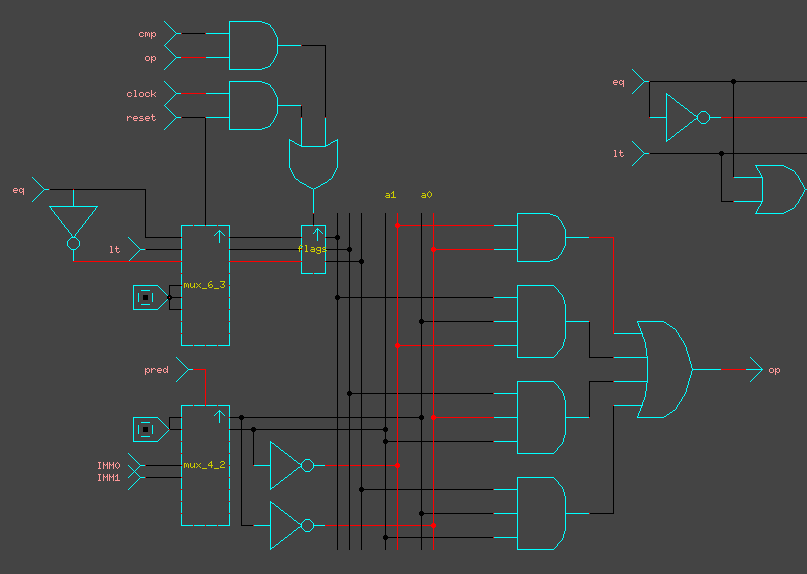
\includegraphics[width=.8 \textwidth]{mgr_cmp}}
\captionof{figure}{Comparaison et calcul du bit \texttt{op}}

\section{Modifications apportées au compilateur}

\subsection{Changement des instructions \texttt{ld} et \texttt{st} en type \texttt{1a}}

\subsubsection{$asm.ml$}
\paragraph{\texttt{instr\_to\_bin}}
On gère le cas où \texttt{i} correspond à \texttt{Load} ou \texttt{Store}, au lieu d'appeler la fonction \texttt{instr\_to\_bin\_type1b}, on appelle la fonction \texttt{instr\_to\_bin\_type1}.
\begin{lstlisting}
	let instr_to_bin = fun i caddr assoc ->
		match i with
		| Load (rd,rs) ->
-			instr_to_bin_type1b 0b100 0 1 rd rs 0
+			instr_to_bin_type1 0b100 0 1 rd rs 0
		| Store (rs,rd) ->
-			instr_to_bin_type1b 0b100 0 0 rd rs 0
+			instr_to_bin_type1 0b100 0 0 rd rs 0
\end{lstlisting}

\subsection{Ajout des instructions \texttt{cmpi} et \texttt{cmp}}

\subsubsection{$lexer.mll$}
\paragraph{\texttt{keyword\_table}}
On ajoute les lignes correspondant aux instructions \texttt{cmpi} et \texttt{cmp} dans la table de hashage \texttt{keyword\_table}.
\begin{lstlisting}
	let keyword_table = Hashtbl.create 53
	let _ =
		List.iter (fun (kwd, tok) -> Hashtbl.add keyword_table kwd tok)
		[
+			"cmpi", CMPI;
+			"cmp",  CMP;
		]
\end{lstlisting}

\subsubsection{$parser.mly$}
\paragraph{\texttt{code}}
On ajoute les lignes correspondant aux instructions \texttt{cmpi} et \texttt{cmp} dans \texttt{code}.
\begin{lstlisting}
	code:
+		| CMPI REG COMA INT	{ assert (-128<=$4 && $4<=127); Cmpi ($2, $4) }
+		| CMP REG COMA REG	{ Cmp ($2, $4) }
	;
\end{lstlisting}

\subsubsection{$asm.ml$ et $asm.mli$}
\paragraph{\texttt{type instr}}
On commence par ajouter \texttt{Cmpi} et \texttt{Cmp} au type \texttt{instr}.
\begin{lstlisting}
	type instr =
+		| Cmpi  of (int * int)			(** rd, uimm8		*)
+		 Cmp   of (int * int * int)		(** rs, rt, pred	*)
\end{lstlisting}
\paragraph{\texttt{dump\_instr}}
On ajoute les cas correspondant aux instructions \texttt{cmpi} et \texttt{cmp} pour afficher leur résultat sur sortie standard.
\begin{lstlisting}
	let dump_instr = fun i -> match i with
+	| Cmpi (rd, v) ->
+		Printf.printf "flags <- cmp(r%d,%d)\n" rd v
+	| Cmp (rs, rt) ->
+		Printf.printf "flags <- cmp(r%d,r%d) (%d)\n" rs rt
\end{lstlisting}
\paragraph{\texttt{instr\_to\_bin}}
On ajoute les cas correspondant aux instructions \texttt{cmpi} et \texttt{cmp}. On appelle alors respectivement les fonctions \texttt{instr\_to\_bin\_type2} et \texttt{instr\_to\_bin\_type1} qui les transformera en compte compris par $Diglog$.
\begin{lstlisting}
	let instr_to_bin = fun i caddr assoc ->
		match i with
+		| Cmpi (rd,v) ->
+			instr_to_bin_type2 0b011 1 0 rd v
+		| Cmp (rs,rt) ->
+			instr_to_bin_type1 0b011 1 1 0 rs rt
\end{lstlisting}

\subsection{Gestion des prédicats}

\subsubsection{$parser.mly$}
\paragraph{\texttt{code}}
Pour chaque ligne traîtant une instruction de type \texttt{1a}, on la modifie pour que la fonction qu'elle appelle prenne un paramètre de type \texttt{int} en plus, qu'on initialise à 0. De plus, Pour chacune de ces lignes, on en crée une nouvelle qui nous permettra d'indique un prédicat pouvant aller de 0 à 3 (entier), et qui permettra au compilateur de l'ajouter dans les instructions concernées.
\begin{lstlisting}
	code:
+		| ADD REG COMA REG COMA REG COMA INT
				{ assert (0<=$8 && $8<=3); Add ($2,$4,$6,false,$8)	}
-		| ADD REG COMA REG COMA REG		{ Add  ($2,$4,$6,false)		}
+		| ADD REG COMA REG COMA REG		{ Add  ($2,$4,$6,false,0)	}
+		| SUB REG COMA REG COMA REG COMA INT
				{ assert (0<=$8 && $8<=3); Add ($2,$4,$6,true,$8)	}
-		| SUB REG COMA REG COMA REG		{ Add  ($2,$4,$6,true)		}
+		| SUB REG COMA REG COMA REG		{ Add  ($2,$4,$6,true,0)	}
+		| CMP REG COMA REG COMA INT
				{ assert (0<=$6 && $6<=3); Cmp ($2, $4, $6)			}
-		| CMP REG COMA REG				{ Cmp ($2, $4)				}
+		| CMP REG COMA REG				{ Cmp ($2, $4, 0)			}
+		| LD REG COMA REG COMA INT
				{ assert (0<=$6 && $6<=3); Load ($2, $4, $6)		}
-		| LD REG COMA REG				{ Load ($2, $4)				}
+		| LD REG COMA REG				{ Load ($2, $4, 0)			}
+		| MOV REG COMA LPAR REG RPAR COMA INT
				{ assert (0<=$8 && $8<=3); Load ($2, $5, $8)		}
-		| MOV REG COMA LPAR REG RPAR	{ Load ($2, $5)				}
+		| MOV REG COMA LPAR REG RPAR	{ Load ($2, $5, 0)			}
+		| ST REG COMA REG COMA INT		{ Store ($4, $2, $6)		}
-		| ST REG COMA REG				{ Store ($4, $2)			}
+		| ST REG COMA REG				{ Store ($4, $2, 0)			}
+		| MOV LPAR REG RPAR COMA REG COMA INT
				{ assert (0<=$8 && $8<=3); Store ($3, $6, $8)		}
-		| MOV LPAR REG RPAR COMA REG	{ Store ($3, $6)			}
+		| MOV LPAR REG RPAR COMA REG	{ Store ($3, $6, 0)			}
	;
\end{lstlisting}

\subsubsection{$asm.ml$}
\paragraph{\texttt{instr\_to\_bin\_type1}}
On modifie la fonction pour qu'elle puisse prendre en paramètre un prédicat \texttt{p}, qu'elle ajoutera ensuite au code de l'instruction.
\begin{lstlisting}
-	let instr_to_bin_type1 = fun c f1 f2 r1 r2 r3 ->
+	let instr_to_bin_type1 = fun c f1 f2 r1 r2 r3 p ->
		let hi = (c lsl 5) + (f1 lsl 4) + (f2 lsl 3) + r1 in
-		let lo = (r2 lsl 5) + (r3 lsl 2) in
+		let lo = (r2 lsl 5) + (r3 lsl 2) + p in
		(Printf.sprintf "%02x" hi, Printf.sprintf "%02x" lo)
\end{lstlisting}
\paragraph{\texttt{instr\_to\_bin}}
Les instructions gérées par la fonction prennent maintenant en compte les prédicats
\begin{lstlisting}
	let instr_to_bin = fun i caddr assoc ->
		match i with
-		| Add (rd,rs,rt,b) ->
-			let f1 = if b then 1 else 0 in
-			instr_to_bin_type1 0b010 f1 1 rd rs rt
+		| Add (rd,rs,rt,b,p) ->
+			let f1 = if b then 1 else 0 in
+			instr_to_bin_type1 0b010 f1 1 rd rs rt p
-		| Cmp (rs,rt) ->
-			instr_to_bin_type1 0b011 1 1 0 rs rt
+		| Cmp (rs,rt,p) ->
+			instr_to_bin_type1 0b011 1 1 0 rs rt p
-		| Load (rd,rs) ->
-			instr_to_bin_type1 0b100 0 1 rd rs 0
+		| Load (rd,rs,p) ->
+			instr_to_bin_type1 0b100 0 1 rd rs 0 p
-		| Store (rs,rd) ->
-			instr_to_bin_type1 0b100 0 0 rd rs 0
+		| Store (rs,rd,p) ->
+			instr_to_bin_type1 0b100 0 0 rd rs 0 p
\end{lstlisting}

\section{Codes de tests}

\subsection{Vérification du fonctionnement des prédicats}
\lstinputlisting{../asm/1.asm}

\subsection{Vérification de l'instruction \texttt{cmp}}
\lstinputlisting{../asm/2.asm}

\subsection{Vérification des instructions \texttt{in} et \texttt{out}}
\lstinputlisting{../asm/3.asm}

\subsection{Vérification des instructions de saut conditionnel}
\lstinputlisting{../asm/4.asm}

\end{document}
